%! TeX program = lualatex
\documentclass[10pt,a4paper,table]{article}

\usepackage{amsmath,amssymb,amsthm,mathtools,amsfonts}
\usepackage{breqn}
\usepackage[utf8]{inputenc}
\usepackage[danish]{babel}
\usepackage[T1]{fontenc}

%%%%%%%%%%%%%%%%%%%%%%%%%%%%%%%%%%%%%%%%%%%%%%%%%%%%%%%%%%%%%%%%%%%%%%%%%%%%%% Fonts

\usepackage{fontspec}
\setmainfont{Times New Roman}
\newfontfamily\garamond[Numbers=OldStyle]{EB Garamond}
\newfontfamily\plantin[Numbers=OldStyle]{Plantin MT Pro}
\newfontfamily\quotefont[Ligatures=TeX]{Linux Libertine O}
\newfontfamily\vest{TRY Vesterbro Regular}
\newfontfamily\vestb{TRY Vesterbro Poster}
\newfontfamily\overp{Overpass}

%%%%%%%%%%%%%%%%%%%%%%%%%%%%%%%%%%%%%%%%%%%%%%%%%%%%%%%%%%%%%%%%%%%%%%%%%%%%%% Colors

\usepackage{xcolor}
\usepackage{transparent}

\definecolor{frbblue}{RGB}{47, 88, 109}
\definecolor{hgred}{RGB}{140, 10, 10}
\definecolor{frbgreenl}{RGB}{162, 202, 137}
\definecolor{frbgreen}{RGB}{28, 85, 66}
\definecolor{frbgrey}{RGB}{243, 245, 242}
\definecolor{postityellow}{RGB}{255, 242, 153}
\definecolor{postitgreen}{RGB}{204, 235, 197}
\definecolor{postitblue}{RGB}{199, 224, 244}
\definecolor{postitpink}{RGB}{248, 203, 214}

%%%%%%%%%%%%%%%%%%%%%%%%%%%%%%%%%%%%%%%%%%%%%%%%%%%%%%%%%%%%%%%%%%%%%%%%%%%%%% Other Graphics

\usepackage{graphicx}
\graphicspath{{../img/}}
\usepackage{tikz}
\usetikzlibrary{calc,shadows}
\usepackage{placeins}

\usepackage[pdfborder={0 0 0}]{hyperref}

\usepackage{multicol}
\usepackage{cellspace}
\setlength\cellspacetoplimit{100pt}
\setlength\cellspacebottomlimit{100pt}
\usepackage{tabularx}
\newcolumntype{b}{>{\hsize=\hsize}>{\centering\arraybackslash}X}
\usepackage{siunitx}
\setlength\cellspacetoplimit{4pt}
\setlength\cellspacebottomlimit{4pt}

\usepackage{enumitem}
\usepackage{wrapfig}
\usepackage{caption}
\usepackage{titlesec}

\setlength{\parskip}{0.5\baselineskip}
\setlength{\parindent}{0cm}
\setlist[enumerate]{label=\alph*),left=20pt}

%%%%%%%%%%%%%%%%%%%%%%%%%%%%%%%%%%%%%%%%%%%%%%%%%%%%%%%%%%%%%%%%%%%%%%%%%%%%%% New commands

\newcommand\svar[1]{\newline\textcolor{red}{\textbf{Svar}\\#1}}

\newcommand*\quotesize{20}
\newcommand*{\openquote}
  {\tikz[remember picture,overlay,xshift=-3ex,yshift=-0ex]
    \node (OQ) {\quotefont\fontsize{\quotesize}{\quotesize}\selectfont``};\kern0pt}

\newcommand*{\closequote}[1]
  {\tikz[remember picture,overlay,xshift=2ex,yshift={#1}]
    \node (CQ) {\quotefont\fontsize{\quotesize}{\quotesize}\selectfont''};}

\newcommand{\qm}[1]{``#1''}
\newcommand{\iquote}[1]{\begin{quote}\itshape \openquote#1\hfill\closequote{0ex} \end{quote}}

%%%%%%%%%%%%%%%%%%%%%%%%%%%%%%%%%%%%%%%%%%%%%%%%%%%%%%%%%%%%%%%%%%%%%%%%%%%%%% Sections
\usepackage{chngcntr}

\renewcommand\thesection{\arabic{section}}

\titleformat{\section}[block]
  {\flushright\overp\Large\color{frbgreen}}
  {}
  {0pt}
  {\clearpage EKSTRA}
  [{\color{frbgreenl}\vspace{-1em}\hspace*{-0.165\linewidth}\rule{\dimexpr1.165\linewidth\relax}{0.4pt}\kern1mm}]

\counterwithout{subsection}{section}
\renewcommand\thesubsection{Exercise \arabic{subsection}}
\titleformat{\subsection}[leftmargin]{\bfseries}{}{0pt}{\hspace{-5em}\thesubsection}

%%%%%%%%%%%%%%%%%%%%%%%%%%%%%%%%%%%%%%%%%%%%%%%%%%%%%%%%%%%%%%%%%%%%%%%%%%%%%% Header & Footer

\usepackage{bigfoot}
\DeclareNewFootnote{a}
\renewcommand{\thefootnotea}{\fnsymbol{footnotea}}
\newcommand{\footnotes}[1]{\footnotea[2]{#1}}
\MakePerPage{footnotes}

\usepackage{fancyhdr}
\fancypagestyle{plain}{%
  \setlength{\headheight}{60pt}%
  \setlength{\headsep}{0pt}
  \fancyhf{}
  \renewcommand{\footrulewidth}{0pt}%
  \renewcommand\headrule{}%
  \fancyhead[L]{}
  \fancyhead[C]{}
  \fancyhead[R]{\overp\color{frbgreenl}\normalsize English\\\huge\color{frbgreen}\vestb The Doll's House}
  \cfoot{\thepage}
}
\pagestyle{fancy}
\fancyhf{}
\renewcommand\headrule{}
\lhead{}
\rhead{}
\cfoot{\thepage}

%%%%%%%%%%%%%%%%%%%%%%%%%%%%%%%%%%%%%%%%%%%%%%%%%%%%%%%%%%%%%%%%%%%%%%%%%%%%%% Document

\begin{document}
\thispagestyle{plain}
\begin{tikzpicture}[remember picture,overlay]
    \node[anchor=north west,yshift=-48pt,xshift=120pt,opacity=0.2]%
        at (current page.north west)
        {
\includegraphics[scale=0.25]{frbvuc_logo.png}};
\end{tikzpicture}
\begin{tikzpicture}[remember picture,overlay]
  \definecolor{bgline}{RGB}{205,214,208}
  \coordinate (C) at ($(current page.north)+(35mm,-5mm)$);
  \draw[bgline, line width=0.6pt] (C) circle (65mm);
  \draw[bgline, line width=0.4pt]
    ($(current page.north east)+(0,0mm)$) ++(-28mm,0)
    -- ($(current page.south east)+(0,10mm)$) ++(-28mm,0);
\end{tikzpicture}

\subsection{}

\textbf{Find a superordinate term for each of these categories.}

\vspace{0.3cm}

\begin{enumerate}[label=\alph*),left=20pt,itemsep=1em]
  \item \textcolor{purple}{\textbf{\textit{accepted $\cdot$ approved $\cdot$ favourite $\cdot$ in demand}}}\\[0.5em]
  \rule{0.55\textwidth}{0.4pt}
  \item \textcolor{purple}{\textbf{\textit{shut out $\cdot$ ban $\cdot$ reject $\cdot$ prohibit}}}\\[0.5em]
  \rule{0.55\textwidth}{0.4pt}
  \item \textcolor{purple}{\textbf{\textit{embrace $\cdot$ involve $\cdot$ take in $\cdot$ incorporate}}}\\[0.5em]
  \rule{0.55\textwidth}{0.4pt}
  \item \textcolor{purple}{\textbf{\textit{alien $\cdot$ stranger $\cdot$ intruder $\cdot$ interloper}}}\\[0.5em]
  \rule{0.55\textwidth}{0.4pt}
\end{enumerate}

\clearpage
\subsection{}
\enlargethispage{1.5cm}

\textbf{Match the definitions with the correct words.}\\[-0.2em]
{\small Draw a line from each definition on the left to the matching word on the right.}

\vspace{0.25cm}

\begin{tikzpicture}[
  def/.style={draw=frbgreenl, rounded corners=3pt, align=left, text width=0.52\textwidth, inner sep=3pt, font=\scriptsize, anchor=west},
  word/.style={draw=frbgreenl, rounded corners=3pt, align=center, text width=0.18\textwidth, inner sep=4pt, font=\scriptsize\bfseries, anchor=west},
  dot/.style={circle, draw=frbgreen, fill=white, inner sep=1.3pt}
]
  % Definitions
  \node[def] (d1)  at (0,0)       {1. unity or agreement of feeling or action, especially among individuals with a common interest; mutual support within a group};
  \node[def] (d2)  at (0,-1.3)    {2. the ability to identify oneself mentally with someone else and so to understand that person's feelings};
  \node[def] (d3)  at (0,-2.55)   {3. the act of deliberately not including somebody in a group or activity. The first letter is O};
  \node[def] (d4)  at (0,-3.75)   {4. principles or standards of behaviour; one's judgement of what is important in life};
  \node[def] (d5)  at (0,-4.85)   {5. lack of guile or corruption; purity; blamelessness};
  \node[def] (d6)  at (0,-5.85)   {6. seek to harm, intimidate, or coerce someone perceived as vulnerable};
  \node[def] (d7)  at (0,-6.95)   {7. practical contact with and observation of facts or events; an event or occurrence which leaves an impression on someone};
  \node[def] (d8)  at (0,-8.3)    {8. the acceptance of something undesirable but inevitable};
  \node[def] (d9)  at (0,-9.3)    {9. preconceived opinion that is not based on reason or actual experience};
  \node[def] (d10) at (0,-10.45)  {10. the faculty or action of forming new ideas, images, or concepts of external objects not present to the senses};
  \node[def] (d11) at (0,-11.8)   {11. the superior attitude or behaviour associated with a certain part of society};
  \node[def] (d12) at (0,-12.95)  {12. a feeling of expectation and desire for a particular thing to happen};
  \node[def] (d13) at (0,-14.05)  {13. the expression of one's meaning by using language that normally signifies the opposite, typically for humorous or emphatic effect};
  \node[def] (d14) at (0,-15.55)  {14. a strong desire or craving for something (originally associated with food)};

  % Words (mixed order)
  \node[word] (w1)  at (9.15,0)       {moral};
  \node[word] (w2)  at (9.15,-1.2)    {bully};
  \node[word] (w3)  at (9.15,-2.4)    {solidarity};
  \node[word] (w4)  at (9.15,-3.6)    {experience};
  \node[word] (w5)  at (9.15,-4.8)    {empathy};
  \node[word] (w6)  at (9.15,-6.0)    {innocence};
  \node[word] (w7)  at (9.15,-7.2)    {ostracism};
  \node[word] (w8)  at (9.15,-8.4)    {yearning};
  \node[word] (w9)  at (9.15,-9.6)    {irony};
  \node[word] (w10) at (9.15,-10.8)   {hope};
  \node[word] (w11) at (9.15,-12.0)   {resignation};
  \node[word] (w12) at (9.15,-13.2)   {snobbery};
  \node[word] (w13) at (9.15,-14.4)   {imagination};
  \node[word] (w14) at (9.15,-15.6)   {prejudice};

  % Connection points
  \foreach \n in {d1,d2,d3,d4,d5,d6,d7,d8,d9,d10,d11,d12,d13,d14} {
    \node[dot] at (\n.east) {};
  }
  \foreach \n in {w1,w2,w3,w4,w5,w6,w7,w8,w9,w10,w11,w12,w13,w14} {
    \node[dot] at (\n.west) {};
  }
\end{tikzpicture}

\clearpage
\subsection{}

\begin{enumerate}[label=\arabic*.,left=20pt,itemsep=0.8em]
  \item \textbf{QUOTATIONS.} Read the last part of the text, and, as you read, comment on the quotations below. Also add two quotations from the text which you find important and explain their meaning in the text and your reaction to them.
  \item Which symbols can you find in the text? Write them down and connect them with quotations from the text. What do they signify?
\end{enumerate}

\vspace{0.2cm}

{\small
\renewcommand{\arraystretch}{1.7}
\setlength{\tabcolsep}{3pt}
\noindent\begin{tabularx}{0.94\textwidth}{|>{\raggedright\arraybackslash}p{0.50\textwidth}|>{\raggedright\arraybackslash}X|>{\raggedright\arraybackslash}X|}
  \hline
  \textbf{Quotation} & \textbf{Meaning in the text} & \textbf{Your reaction} \\
  \hline
  \textit{... while they chewed their jam sandwiches out of a newspaper} & & \\
  \hline
  \textit{``Run away Kezia; you know very well why not.''} & & \\
  \hline
  \textit{And never did they skip so high, run in and out so fast, or do such daring things as on that morning.} & & \\
  \hline
  \textit{``You can come in and see our doll's house''} & & \\
  \hline
  \textit{``Your ma told our ma you wasn't to speak to us.''} & & \\
  \hline
  \textit{``Kezia!''} & & \\
  \hline
  \textit{The afternoon had been awful. ... Those little rats of Kelveys.} & & \\
  \hline
  \textit{``I seen the little lamp,''} & & \\
  \hline
  \rule{0pt}{1.2cm} & & \\
  \hline
  \rule{0pt}{1.2cm} & & \\
  \hline
\end{tabularx}
}

\end{document}

